\subsection{Interface thérapeutique pour l'ajustement de la difficulté de serious games}	
\emph{Hammer \& Planks} est, dans sa version thérapeutique, un jeu permettant d'aider à récupérer des facultés motrices dans le cadre d'un accompagnement à la rééducation. Rappelons qu'il s'agit d'un shooter à défilement vertical dans lequel le joueur contrôle un bateau qu'il dirige avec des mouvements du corps. Le joueur doit éviter des obstacles, affronter divers ennemis et ramasser des bonus sur la mer. Tous ces objets possèdent des attributs qu'il est possible de modifier afin d'adapter le jeu aux besoins et aux capacités du patient. Ce fut mon travail durant la première partie de mon stage de permettre de modifier ces paramètres directement à partir d'une interface web contrôlée par le soignant menant la séance de thérapie.
\paragraph{}
Ce projet se divise en deux parties distinctes~:
\begin{enumerate}
	\item L'interface thérapeutique
	\item Le paramétrage des variables de jeu
\end{enumerate}

	\subsubsection*{Interface thérapeutique}
Celle-ci permet, à partir d'un terminal distinct, de choisir un jeu et de lancer une partie sur le terminal utilisé par le patient (voir figure~\ref{interface_accueil}). Celui-ci sera équipé d'un périphérique de contrôle comme la caméra Kinect ou la wii board. A partir de cette interface, le soignant est en mesure de voir (figure~\ref{ensemble_parametres}) et de modifier(figure~\ref{interface_parametres}) l'ensemble des paramètres de jeu (en tout cas, le sous-ensemble considéré comme pertinent et effectivement envoyé à l'application). 
\begin{figure}[!hbtp]
	\begin{minipage}{0.48\linewidth}	
		\centering
		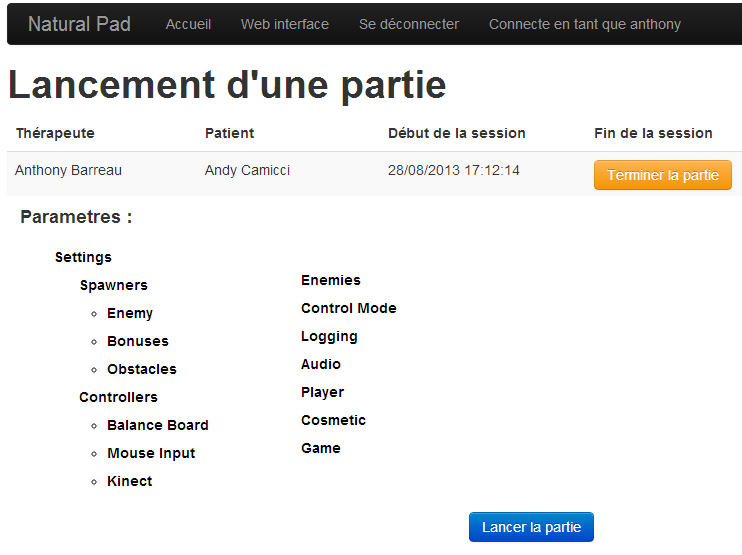
\includegraphics[width=7cm, height=5cm]{images/interface_accueil.png}
		\caption{Interface thérapeutique au lancement d'une partie de H\&P }
		\label{interface_accueil}
	\end{minipage}	
	\begin{minipage}{0.48\linewidth}	
		\centering
		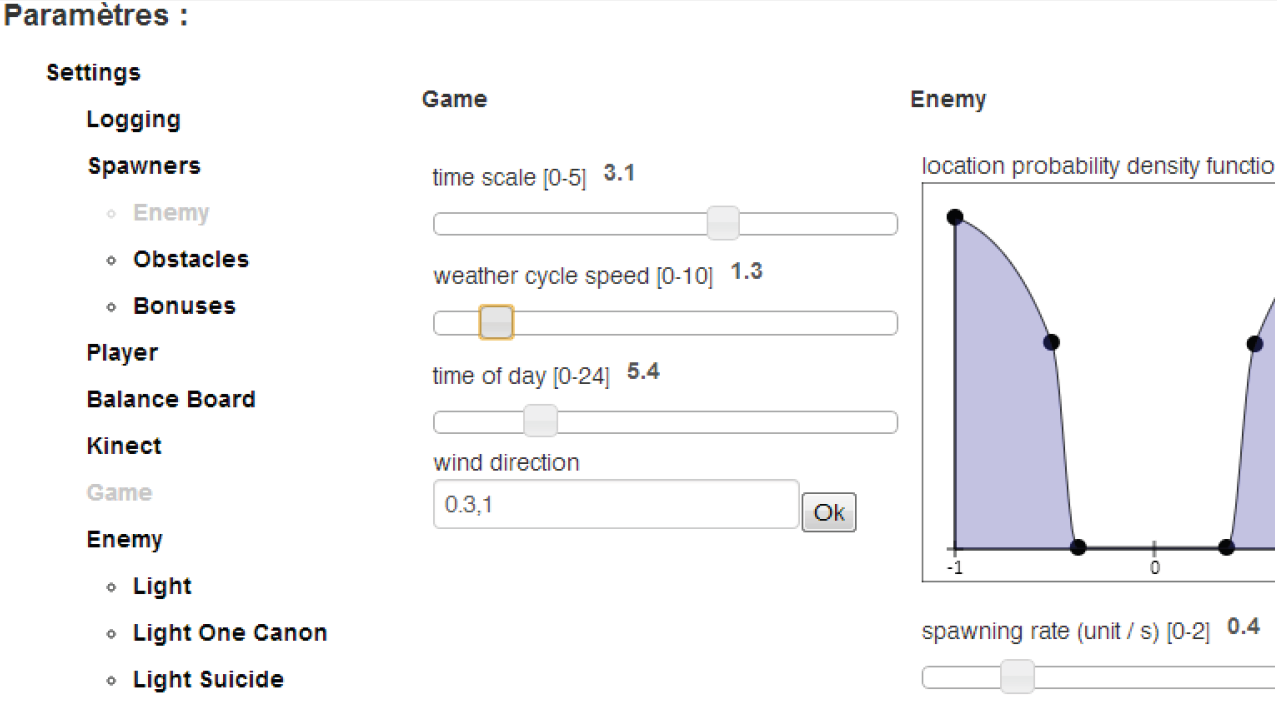
\includegraphics[width=7cm, height=5cm]{images/interface_parametres.png}
		\caption{Modifications de valeurs des paramètres du jeu H\&P}
		\label{interface_parametres}
	\end{minipage}
\end{figure}

\paragraph{} De plus, à la fin d'une partie, il sera capable de visualiser les données de la session de jeu (voir figure~\ref{interface_recap}), comme l'apparition d'évènements ou les zones que le joueur a réussi ou non à atteindre. Ces informations sont utiles pour mieux cibler les difficultés du patient et ajuster au mieux les prochaines séances. Cette partie du projet a été réalisée par Andy Camicci durant son stage chez NaturalPad entre Avril et Juin 2013.
\begin{figure}[!hbtp]
	\centering
		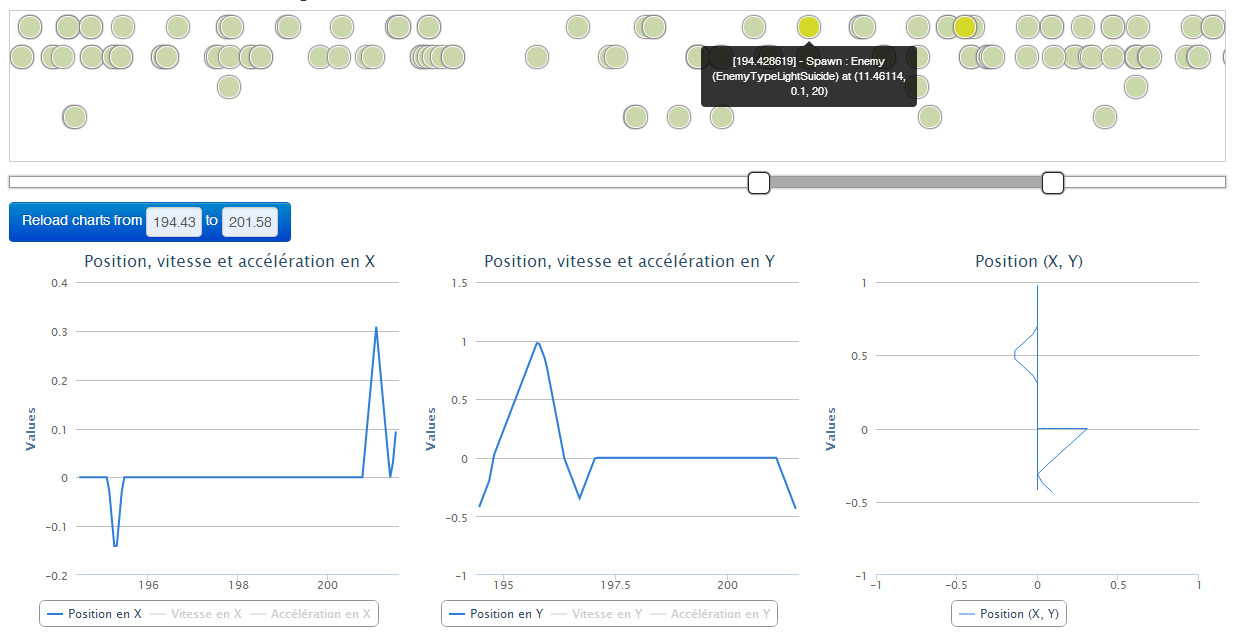
\includegraphics[width=8cm]{images/interface_recap.png}
		\caption{Récapitulatif d'une session de jeu H\&P}
		\label{interface_recap}
\end{figure}


	\subsubsection*{Maitriser la difficulté : le paramétrage des variables de jeu}
Cette partie consiste en l'extraction des paramètres de jeux et en la création d'un système permettant de créer, d'enregistrer et de transmettre des configurations de ces attributs à l'interface thérapeutique.

\paragraph{}
\emph{Hammer \& Planks} est développé avec le moteur de jeu Unity3d et les scripts codés avec le langage de programmation C\#. Comme nous l'avons dit, \emph{H\&P} possède de nombreux contenus contribuant à la richesse du gameplay et aux possibilités d'ajustement. Lors de mon arrivée au sein de NaturalPad, ces objets n'étaient cependant pas ajustables facilement : il fallait rechercher l'ensemble des objets dont on souhaitait modifier un paramètre, trouver les variables correspondant à ces paramètres puis les modifier soit directement dans le code soit par l'intermédiaire de l'éditeur d'Unity. La raison en est que les contraintes de développement du jeu n'ont pas permis de découpler ces informations.

\paragraph{}
Mon premier travail a donc été de découvrir le code et de rechercher toutes les variables dont on souhaiterait potentiellement vouloir modifier la valeur dans un contexte d'ajustement du jeu pour un exercice de rééducation. J'ai ensuite créé une classe spécifique permettant de regrouper conceptuellement les données modifiables. J'ai ainsi regroupé ces données dans des thèmes tels que \emph{réseau}, \emph{ennemis}, \emph{joueur}, \emph{contrôles} ou \emph{cosmétiques} (figure~\ref{ensemble_parametres}).
\begin{figure}[!hbtp]
	\centering
	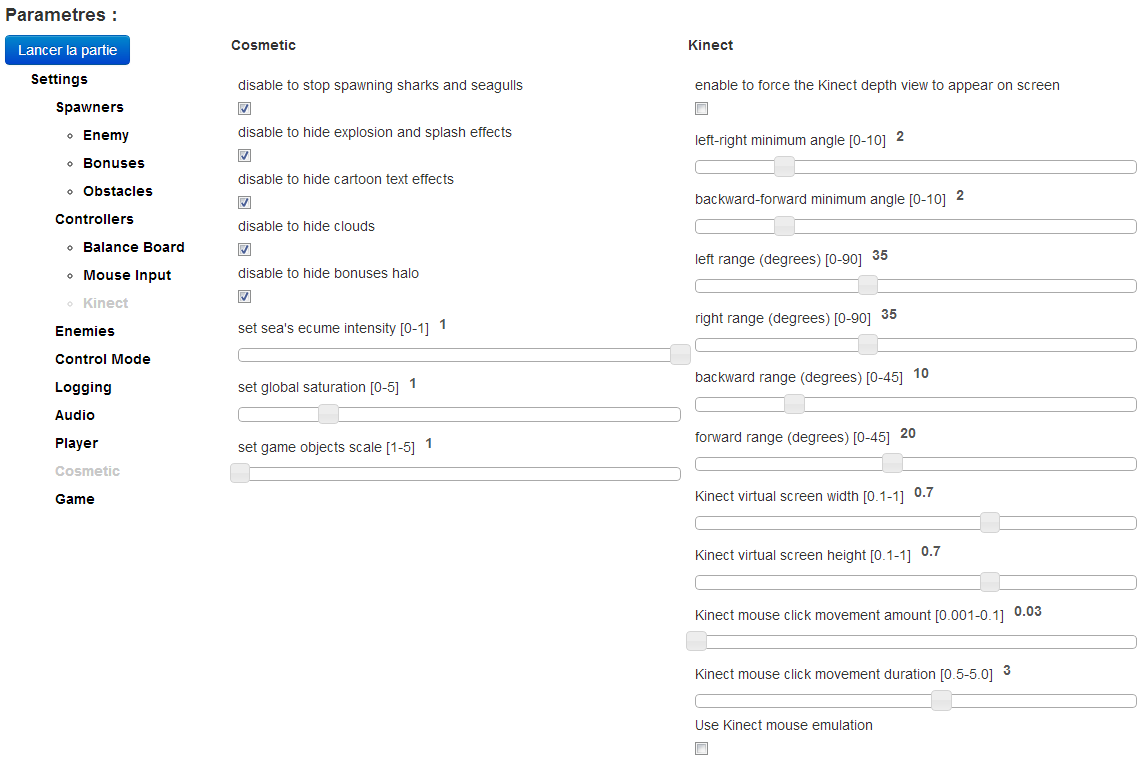
\includegraphics[width=14cm, height=8cm]{images/ensemble_parametres.png}
	\caption{Visualisation des groupes de paramètres dans l'interface web}
	\label{ensemble_parametres}
\end{figure}

\paragraph{}
En parallèle, j'ai aussi procédé au refactoring de l'ensemble des classes possédant ou utilisant un ou plusieurs attributs modifiables. L'intérêt était bien sur d'avoir un accès commun unique à ces valeurs, mais aussi et surtout que les valeurs puissent être modifiées de manière extérieure par l'interface thérapeutique. On peut voir le lien entre la modification des valeurs des paramètres dans l'interface thérapeute et les éléments du jeu en figure~\ref{comparatif_interface_rochers}. Par ailleurs, la modification de ces valeurs par l'interface devait être certaine et pérenne, afin que les modifications apportées soit effectivement prises en compte par l'application et donc modifier l'expérience de jeu en direct.

\begin{figure}[!hbtp]
	\centering
	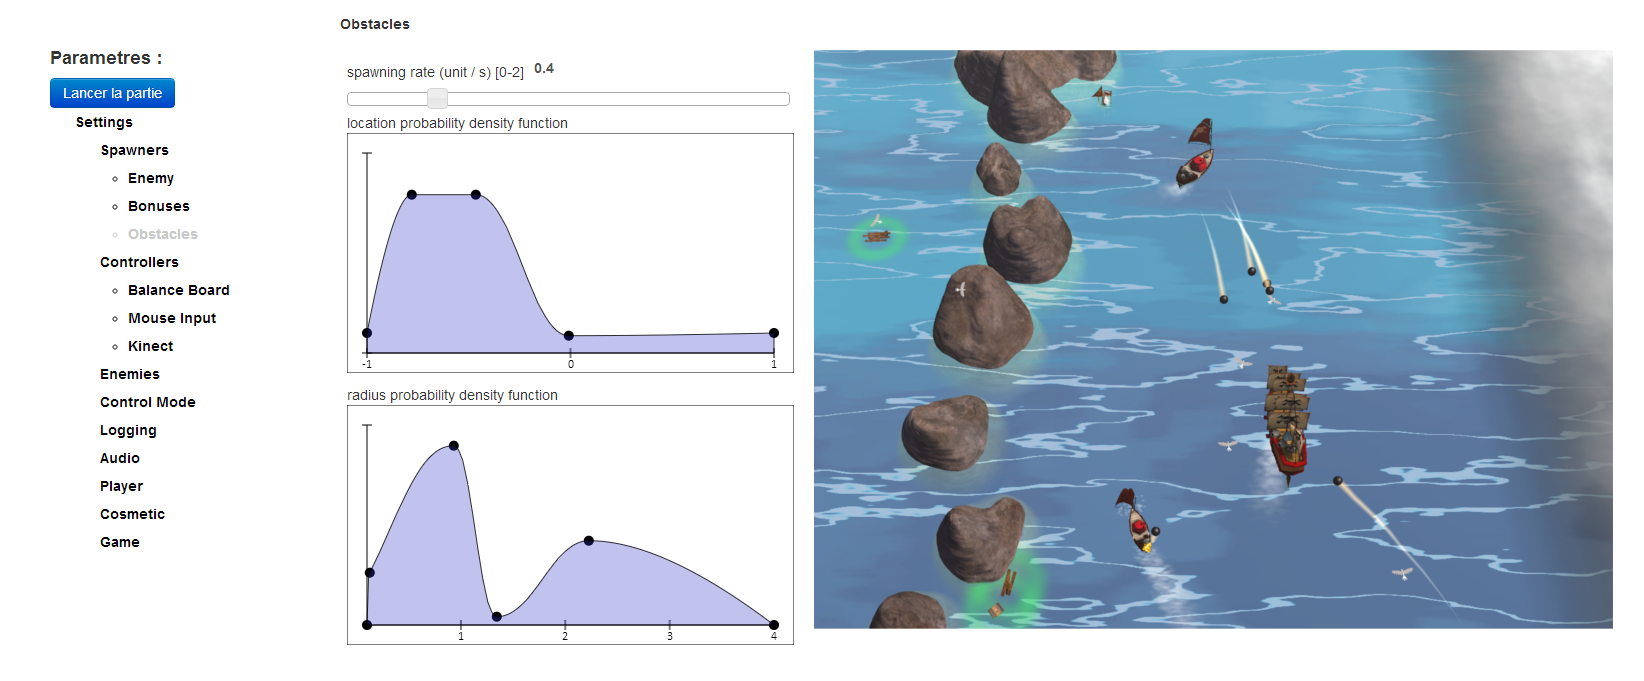
\includegraphics[width=16cm]{images/comparatif_interface_rochers.png}
	\caption{Interface thérapeutique et écran du jeu hammer \& Planks}
\emph{	On voit que le thérapeute a changé la fonction de localisation des rochers dans l'interface, et que cela s'applique dans le jeu. Le patient est ainsi contraint de se diriger sur sa droite, l'incitant à faire travailler son coté hémiplégique.}
	\label{comparatif_interface_rochers}
\end{figure}

	\subsubsection*{Préparer l'évolution du jeu et de la séance}
Si permettre un ajustement en direct des propriétés du jeu par le soignant était une fonctionnalité que nous voulions impérativement mettre en place, celle-ci peut se révéler contraignante et répétitive si elle est utilisée seule. Nous voulions aussi enregistrer des configurations de paramètres, afin de pouvoir passer de l'une à l'autre aisément sans devoir faire chaque modification séparément. Par ailleurs, cela permet d'envisager beaucoup de possibilités comme la personnalisation de configurations pour des patients, l'adaptation aisée du jeu pour des besoins thérapeutiques différents ou encore l'automatisation d'une progression de la difficulté à l'aide de configuration prédéfinies.

\paragraph{}Afin d'utiliser des fichiers de configurations, il a fallu créer un système permettant de serialiser les données puis de les charger et de les lier à l'instance de jeu.\\
J'ai par ailleurs durant mon stage créé plusieurs fichiers de configuration permettant une évolution progressive de la difficulté dans le mode de jeu Survie de \emph{Hammer \& Planks}, pour sa version grand public.

	\subsubsection*{Usage : tests, retours et intégrations}
Si le projet \emph{Hammer \& Planks} a été initié par une étudiante en ergothérapie, il est aussi développé en collaboration avec le pôle de rééducation du centre hospitalier de Lapeyronie à Montpellier. Comme nous l'avons dit, le projet a évolué et son champs d'action, en plus d'un travail sur l'équilibre, s'étend maintenant à de l'aide à la rééducation des membres supérieurs, du tronc et du bassin. Le travail d'équilibre, qu'il soit debout ou assis, s'effectue en utilisant la balance de la Wii, qui enregistre les changements du centre de gravité du joueur-patient pour contrôler le bateau. L'intégration d'un contrôle avec la Kinect permet au joueur d'utiliser d'autres mouvements de son corps. Il est ainsi possible d'utiliser son bras ou sa main pour diriger le bateau, ou les mouvements du tronc et du bassin que ce soit en position assise ou debout.

\paragraph{} Nous approchant d'une méthode de conception participative, nous avons ainsi réalisé plusieurs séances de tests avec des patients hémiplégiques et leurs thérapeutes. \\
Les premières choses marquantes sont la curiosité et l'enthousiasme général à la fois des patients et du personnel soignant. Peu d'entre eux connaissaient l'existence de jeux sérieux pour la santé, et dans le cas contraire, appréciaient particulièrement l'accent mis sur l'aspect vidéo-ludique de \emph{Hammer \& Planks}. Ce fut donc un premier point très positif pour l'équipe.
\begin{figure}[hbt]
	\centering
	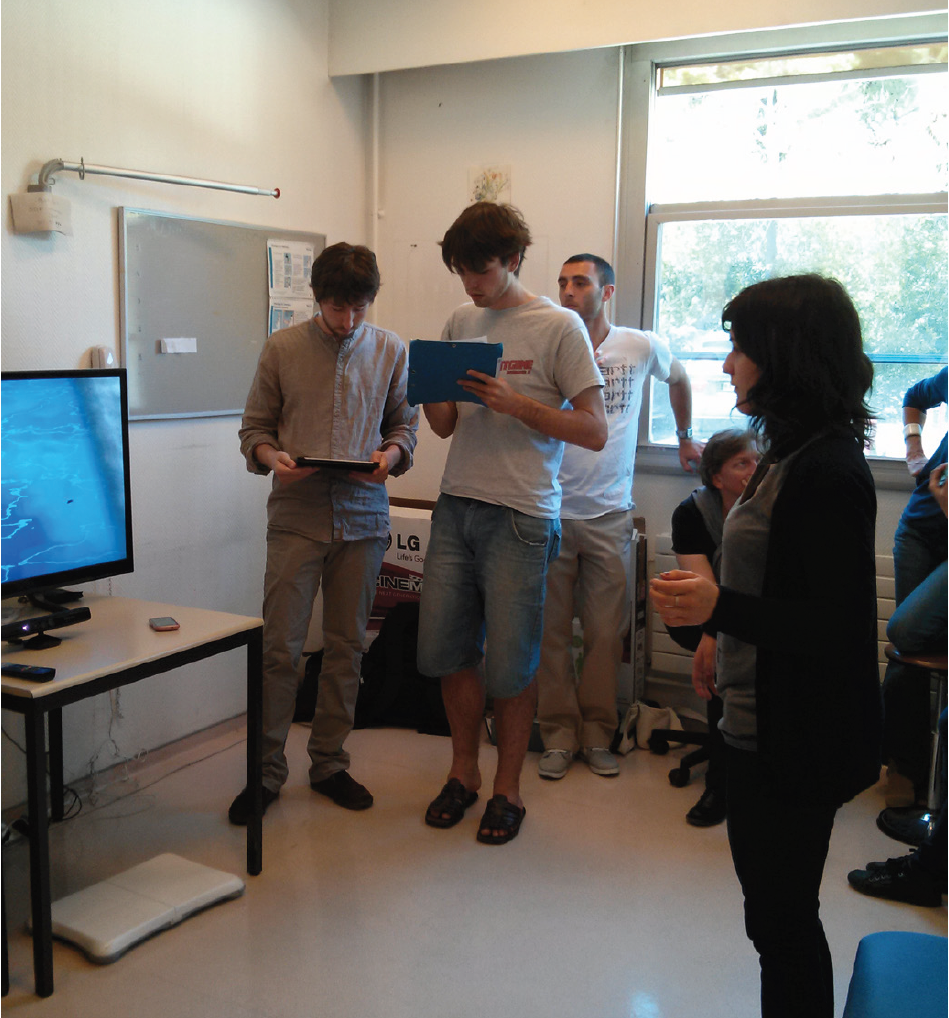
\includegraphics[height=11cm]{images/test_lapeyronie.png}
	\caption{Séance de test du jeu Hammer \& Planks au centre hospitalier de Lapeyronie}
	\label{test_lapeyronie}
\end{figure}
\paragraph{} 
Lors de la première séance de tests, nous avons ainsi eu de nombreux retours positifs portant sur la possibilité d'ajuster le jeu en direct, la visualisation des informations de la session de jeu ou encore le plaisir de jeu. Nous avons aussi eu de nombreuses remarques menant à l'ajout de fonctionnalités, notamment par le personnel.\\
Les remarques les plus fréquentes concernaient le visuel du jeu : les soignants craignaient que les graphismes soient trop riches et les effets trop complexes pour des patients hémiplégiques. L'effet visuel des mouvements de la mer fut notamment cité, et la différenciation entre bonus et obstacles (ennemis, projectiles et mines ennemies) jugée trop complexe.\\
Enfin, réaliser des tests pendant une demie-journée nous a aussi permis de juger le résultat selon d'autres critères. Durant la phase d'ajustement des paramètres via l'interface thérapeutique, certains ajustements revenaient systématiquement, remettant en cause la pertinence de notre configuration par défaut. A l'inverse, certaines valeurs n'étaient jamais utilisées, ni même finalement envisageables : la plage de valeurs de certains paramètres était donc à revoir.

\paragraph{De l'importance des tests utilisateurs\\}Petite anecdote enfin, prouvant définitivement l'importance de réaliser des tests en conditions réelles. Lorsqu'on utilise le jeu avec la Kinect, le joueur doit lever la main afin d'être reconnu comme la personne joueuse parmi les possibles multiples personnes détectées par la caméra. Ce système fonctionnait parfaitement lors de nos tests en interne. Or, quand une patiente hémiplégique a tenté de jouer, le système ne l'a pas reconnue. La raison en était que la patiente avait une hémiplégie du coté gauche et voulait donc jouer avec sa main gauche pour travailler sa rééducation. Or, le système était configuré pour ne détecter qu'une main droite... aucun membre de l'équipe n'étant gaucher, nous n'avions pas détecté ce grossier oubli ! L'erreur a bien sur depuis été corrigée.

	\paragraph{\emph{Intégration}\\}
	Forts de ces retours, nous avons ensuite classé les remarques qui nous ont été faites. Puis, nous avons discuté de la pertinence et de l'importance de chacune d'elles, ainsi que des différentes possibilités d'y répondre. \\
	Concernant la surcharge visuelle, pouvant poser des problèmes cognitifs à certains patients, surtout pour des personnes peu, voir pas, habituées aux jeux vidéo, nous avons mis en place la possibilité d'ajuster les paramètres visuels. Il est possible de modifier le contraste du jeu, la taille des éléments interactifs ou encore de supprimer les objets cosmétiques (requins, mouettes, brouillard, effet de la mer, etc.). Nous avons par ailleurs augmenté la taille des projectiles (ennemis et alliés) et ajouté un effet de trainée, les rendant beaucoup plus visibles.\\
	Concernant les bonus, jugés trop difficiles à ramasser, nous mis en place deux systèmes. Le premier est la possibilité de mettre un halo vert autour des différents bonus, les rendant bien plus visibles. Le second, est un mécanisme d'aimantage des bonus vers le bateau du joueur. Cette attraction, dont le rayon est ajustable dans les settings, permet de récupérer les bonus même si on ne passe pas directement dessus, ce qui est souvent difficile et frustrant pour le joueur.\\
Concernant les paramètres enfin, nous avons modifié les valeurs par défaut de certains et ajusté les bornes min et max des plages de valeurs.

		
	\paragraph{} Nous avons ensuite réalisé une nouvelle séance de tests du jeu intégrant ces modifications. C'est avec plaisir que nous avons constaté que les réponses apportées étaient pertinentes et plaisaient à nos testeurs. Ce fut aussi l'occasion d'avoir de nouveaux retours et de continuer notre processus de conception participative.
	
	\subsubsection*{Conclusion}
	Cette expérience et ce travail sur \emph{Hammer \& Planks} m'ont permis de vérifier l'intérêt et la réelle pertinence de jeux sérieux pour la rééducation. Par ailleurs, l'intégration d'un nouveau périphérique, la Kinect, m'a confirmé l'importance du moyen de contrôle à la fois sur le gameplay mais aussi et surtout sur la richesse des applications thérapeutiques qui en découlent. Enfin, les critiques des soignants et des patients au cours des deux séances de tests m'ont assuré de l'importance et du réel intérêt de pouvoir ajuster manuellement les variables de jeux directement pendant la séance. C'est à la fois très gratifiant pour notre travail et très encourageant pour les possibilités en terme de réhabilitation.
	
\paragraph{}
Cependant, un seul jeu, aussi ajustable soit il, ne peut suffire à répondre à tous les besoins et cas d'utilisation. Pour comprendre cela, on peut décomposer un jeu vidéo en trois couches~:
\begin{enumerate}
	\item le cœur du jeu, qui décrit ses lois, objectifs et règles de fonctionnement. Il est propre au jeu (ou à un type de jeu) et non modifiable.
	\item les variables ajustables, qui ne modifient pas les règles mais définissent entre autres la difficulté.
	\item le gameplay, induit par les deux premiers points ainsi que par les périphériques et méthodes de contrôle utilisés. En général, ces derniers sont pris en compte dès l'établissement du coeur du jeu, certaines associations étant incompatibles.
\end{enumerate}
\paragraph{}
Il est possible de modifier l'expérience de jeu en modifiant la valeur des variables ajustables : c'est ce que nous proposons à l'aide de notre interface thérapeutique. Il est aussi possible d'explorer un gameplay a priori identique avec des contrôleurs différents, rendant ainsi à la fois l'expérience de jeu et les mouvements induits différents.
\\Cependant, même ainsi, un jeu vidéo avec un cœur de jeu propre finit par montrer ses limites en terme d'adaptation. Il est alors nécessaire de proposer d'autres types de jeux vidéo si l'on veut explorer de nouvelles pistes de rééducation.\\
Pour cette raison, toujours dans l'idée d'une adaptation de la difficulté, la suite logique était de proposer une méthode permettant d'aider à la conception de jeux sérieux thérapeutiques.
 
\subsection{Conception}
	La seconde partie de mon travail fut consacrée à la proposition et à l'expérimentation de moyens de conception de jeux vidéo sérieux pour la santé. Pour cela, j'ai emprunté deux approches, répondant à des contextes un peu différents.
	
	\subsubsection{Ensemble d'outils d'aide à la conception de SG} \label{boite_outils}
	La première approche s'inscrit dans une problématique où l'on souhaite créer un serious game dont l'objectif sérieux est de l'ordre de l'aide à la réhabilitation motrice. Il s'agit ici de proposer un outil intégrant un certain nombre de connaissances utiles ou nécessaires à la conception de ce type de jeux. L'idée est de mettre à disposition des documents regroupant un maximum des informations qui seront utiles dans le processus de conception. Cela permettrait aux différents corps de métier impliqués dans le processus de conception d'avoir accès à des connaissances qui leur font défaut et d'avoir une vision globale des éléments en jeu.
	
		\paragraph{}
A la frontière entre conception de jeux vidéo et monde médical, ce travail nécessite la compétence de professionnels de la santé ainsi que d’une expertise du domaine du jeu vidéo.
			\paragraph{\emph{Connaissances médicales}\\}
La première étape consiste à définir et lister les objectifs thérapeutiques que l’on souhaite atteindre, les exercices que proposent les professionnels pour y parvenir, ainsi que les éléments de difficulté qui peuvent être rencontrés dans ces exercices. Ces informations doivent provenir de médecins et de thérapeutes qui vont trouver un intérêt dans l’utilisation ou la prescription de serious games pour la santé. Les informations que j'ai pu recueillir, particulièrement autour de l'AVC, sont regroupées dans la partie~\ref{objectifs_therapeutiques}.

\paragraph{}
Dans le but de faciliter la démarche de conception en fonction d’un objectif thérapeutique particulier, il est aussi intéressant de trouver une méthode classification de ces objectifs qui soit parlante pour les thérapeutes. Dans le cadre de mon stage, je me suis particulièrement concentré sur les aspects moteurs, comme présenté dans la figure~\ref{objectifs_moteurs}. Pour réaliser ce document, je me suis tout d'abord inspiré de mes recherches documentaires et du résultats de mes différents entretiens avec des professionnels de la santé.

\paragraph{}
Dans cette première version, j'avais classé les objectifs thérapeutiques au moyen de trois propriétés : la zone du corps affectée (membres supérieurs, inférieurs, tête, tronc), le membre précisément affecté (main - poignet- avant-bras ou pied - jambe, etc.) et des paramètres propres à ces membres (amplitude, force, vitesse ou durée de mouvements, membre gauche ou droit, etc.). Cependant, cette première version avait l'inconvénient de proposer des éléments différents selon le choix initial alors que d'autres éléments étaient dupliqués.

\paragraph{}J'ai ensuite proposé ma classification à deux kinésithérapeutes (Didier Costeau et Karima Bahkti) afin de voir si elle leur semblait pertinente ou s'ils voyaient des éléments à ajouter ou à modifier. Il s'est en fait avéré que cette classification ne correspondait pas du tout à la manière dont raisonnent les thérapeutes lorsqu'ils établissent les objectifs d'une rééducation. Ce fut donc l'occasion de re-designer cette classification. La version 2 ici proposée en figure~\ref{objectifs_moteurs} a par la suite été revue et validée.

\paragraph{}Par ailleurs, dans la perspective d'étendre la portée de l'outil, j'ai aussi ébauché une proposition de listing d'objectifs thérapeutiques de différents types, présentée dans la figure \ref{objectifs_autres}.

\begin{figure}[hbtp]
	\centering
	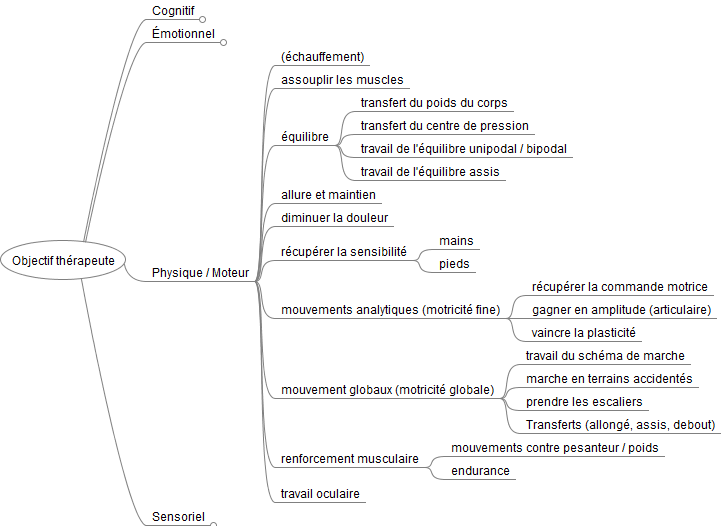
\includegraphics[width=16cm, height=10cm]{images/objectifs_moteurs}
	\caption{Listing et hiérarchisation des objectifs thérapeutiques moteurs}
	\label{objectifs_moteurs}
\end{figure}

\begin{figure}[hbtp]
	\centering
	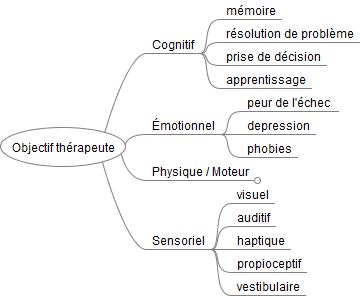
\includegraphics[scale=0.7]{images/objectifs_autres}
	\caption{Ébauche de classification de différentes types d'objectifs thérapeutiques}
	\label{objectifs_autres}
\end{figure}

			\paragraph{\emph{Aspect Game Design}\\}
L'autre aspect du processus de conception de serious games pour la santé concerne l'aspect vidéo-ludique. Pour cela, j'ai établi une classification des principaux types de jeux vidéo en fonction de leur gameplay, proposée dans l'annexe \ref{types_jeux}. Ce document peut être intéressant pour plusieurs raisons. Dans un premier temps, il peut permettre aux concepteurs d'envisager des gameplays auxquels ils n'auraient pas pensé : par oubli ou simplement par méconnaissance du concept de jeu. Pour être plus parlante, la classification propose par ailleurs des exemples de jeux existants pour chaque type de gameplay. \\
Bien sur, cette liste ne peut être totalement exhaustive : beaucoup de jeux vidéo, particulièrement les jeux mettant l'accent sur une difficulté logique, possèdent leur style propre. Le monde des jeux vidéo indépendants regorge par ailleurs de concepts novateurs.

			\paragraph{}
Nous avons vu l'importance des théories cognitives et comportementales dans l'efficacité des jeux sérieux. J'ai aussi fait une proposition de ce que peuvent être les liens et les influences entre ces composantes, suggestion visible sur la figure~\ref{lien_theories}. A partir de ces bases, il me semblait intéressant de proposer une relation entre ces composantes et les \emph{objets} présents dans tout jeux vidéo. Ces objets représentent les feedbacks, les menus, la GUI, les méthodes de contrôle ou les interactions du jeu par exemple. Une proposition générique permettrait de connaître les éléments importants à mettre en place dans le jeu, en fonction de l'élément de théorie sur lequel on souhaite insister. Par exemple, si l'on souhaite concevoir un jeu sérieux pour aider des enfants à se concentrer, on va vouloir mettre en œuvre des éléments indiqués par la théorie de l'engagement et de l'immersion. Il resterait ensuite à trouver quels éléments génériques d'un jeu vidéo permettent d'influencer sur ces éléments.
Cette proposition de lien entre théories cognitives et comportementales et éléments de jeu vidéo, est présentée en annexe~\ref{matching}.

\paragraph{}Malheureusement, il s'est avéré qu'une méthode générique n'était pas appropriée pour répertorier les paramètres d'un jeu vidéo. En fait, chaque type de jeu vidéo à ses règles et mécanismes propres, ce qui modifie radicalement le contenu d'un jeu d'un type à l'autre. Ainsi, dans un jeu d'\emph{aventure graphique point and click}, des éléments comme le contrôle de la vue ou les paramètres d'une partie sont inexistants ou presque, alors qu'ils représentent des éléments essentiels dans les RTS et les FPS.
\paragraph{}A l'inverse, un élément comme le feedback semble particulièrement important quel que soit le type de jeu. Il est par ailleurs en relation avec un grand nombre de ressorts cognitifs. La teneur du besoin n'aura pas une réelle influence sur l'importance de ce paramètre.

\paragraph{}Pour être pertinent, on pourrait proposer le même genre de relation pour plusieurs types de jeux vidéo. Ainsi, une fois défini le type de jeu qu'elle souhaite développer, l'équipe pourrait voir quels sont spécifiquement les éléments sur lesquels elle souhaite insister. \\
Une autre approche serait de pouvoir proposer un type de jeux vidéo à partir d'une sélection de concepts cognitifs ou comportementaux.

			\paragraph{\emph{Le contrôle, lien entre objectifs thérapeutiques et mécanismes ludiques}\\}
Dans notre cadre, l'impact sérieux des serious games étant de nature motrice, nous avons décidé de nous concentrer sur les contrôles. Pour faire le lien entre ces objectifs thérapeutiques et le jeu que l’on veut souhaite pour y répondre, l’utilisation d’interfaces dites naturelles (NUI) nous semblait particulièrement pertinente. 

\paragraph{} 
Théoriquement, les possibilités de mouvements pour interagir avec un jeu sont multiples et variées. Cependant, nous souhaitons nous limiter à l'utilisation de périphériques courants et relativement peu onéreux, c'est-à-dire les périphériques courants du jeu vidéo : accessoires \emph{Wii} et \emph{Kinect}.

\paragraph{} Je me suis concentré sur quelques types de jeux vidéo populaires pour lesquels j'ai réalisé un petit état de l'art des jeux utilisant des mouvements naturels. J'ai réalisé des tests sur différents jeux de \emph{Kinect} et de \emph{Wii} et testé des applications utilisant le \emph{Leap Motion}. \\J'ai par ailleurs étendu cette étude en proposant une adaptation NUI pour des jeux célèbres ou particulièrement représentatifs de leur genre.
La synthèse de ce travail est jointe en annexe~\ref{propositions_controles}. Ce document peut servir de base d'inspiration dans la proposition de contrôles naturels pour des serious games pour la réhabilitation.

	
	\subsubsection{Méthodologie de conception de SG}
	\paragraph{}
La deuxième approche résulte en une méthodologie de conception basée sur une conception participative. 

\paragraph{} La méthode proposée ici s'inspire et conjugue les aspects les plus intéressants pour nos besoins de diverses  méthodes, la co-conception avec les utilisateurs restant les mots clefs de la démarche. Comme nous l'avons vu, c'est une méthode centrée sur l'utilisateur et son rôle actif dans la démarche de conception.

\paragraph{} Durant mon stage, j'ai eu l'occasion de participé à la conception de plusieurs projets à divers moments du processus de conception. Ils serviront ici d'exemple afin d'illustrer les étapes du processus.

	\subsubsection*{Connaître Pourquoi, Qui, Comment et Quoi?}
La première étape de la démarche, si on ne compte pas la prise de contact, consiste à réunir les futurs développeurs, utilisateurs et acteurs de l'application. Ces représentants seront issus de milieux différents et complémentaires afin de posséder l'intégralité des savoirs nécessaires. On cherchera aussi à éviter de sur-représenter un corps de métier ou un type d'acteur plutôt qu'un autre. Durant cette réunion, durant environ 1 à 2 heure, il va falloir répondre à plusieurs questions simples mais fondamentales. On s'inspire ici de l'\emph{impact mapping} pour se focaliser sur les impacts attendus de l'application.

\paragraph{}Pour commencer et durant 15 minutes, chaque participant devra exprimer selon lui quels sont les objectifs de l'application. A chaque prise de parole, l'intervenant marquera l'objectif sur un post-it par exemple, et développera sa pensée oralement avec le groupe. Ces objectifs peuvent être divers et variés : thérapeutiques, financiers, de publication ou marketing par exemple. 

\paragraph{} Pour donner un exemple, la figure~\ref{objectifs_ales} donne les principaux objectifs d'une séance de conception réalisée durant mon stage. Cette séance a eu lieu au Centre hospitalier d'Alès - Cévennes (le CHAC) avec des ergothérapeutes et des kinésithérapeutes, Antoine Seilles et moi-même. L'application envisagée a pour but d'aider des personnes, généralement âgées, étant tombées et ayant peur de rechuter, à remarcher normalement. Les objectifs marqués de rouge sont les objectifs critiques devant être atteints.

\begin{figure}
	\centering
	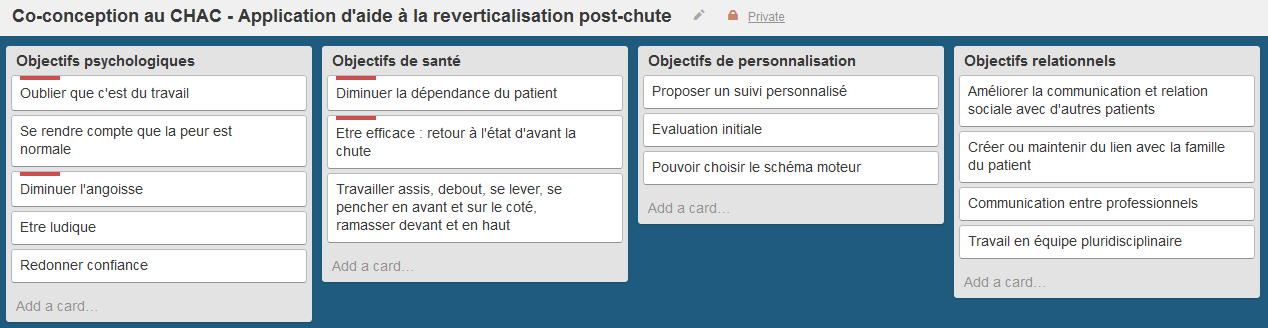
\includegraphics[width = 16cm, height=6cm]{images/objectifs_ales.png}
	\caption{Liste des objectifs issus de la séance de conception sur la verticalisation}
	\label{objectifs_ales}
\end{figure}

\paragraph{} Lorsque le temps est terminé ou qu'aucun nouvel objectif n'est ajouté, une nouvelle période de quinze minutes est lancée. Durant celle-ci, les participants doivent ensemble regrouper les objectifs précédemment énoncés par thème. Enfin, ils doivent choisir un maximum de trois objectifs considérés comme majeurs et principaux. Ce sont sur ces aspects que l'accent devra être mis au cours du processus de conception et de développement.

\paragraph{}En parallèle des deux premières étapes, l'équipe de conception pensera à noter tout utilisateur de l'application. On trouvera dans notre contexte des acteurs comme le patient, sa famille, le kiné, l'ergo ou le médecin par exemple.

\paragraph{}Enfin, on va établir les critères de réussite des objectifs principaux. Comment pourra t-on juger de la réussite ou non de l'application? Existe t-il des références sur lesquelles se baser? Ces critères peuvent concerner des aspects comme le temps, le cout, l'efficacité, la durée, la renommée d'un journal, une valeur de revenue, etc.

	
	\subsubsection*{Comprendre les utilisateurs}
La première partie de la séance de conception participative se concentre sur les objectifs et les impacts de l'application. Dans la seconde partie, on va maintenant se rapprocher 	des utilisateurs. Pour cela, les participants vont devoir imaginer une personne utilisatrice de l'application. Cette méthode permet de simuler un cas concret d'utilisation de l'application en rendant l'expérience bien plus crédible et vivante qu'avec l'impersonnel "utilisateur x". Il s'agit ici de s'inspirer d'une méthode marketing en créant une carte d'empathie.

\paragraph{} Cette carte d'empathie va nous permettre de dresser le profil de l'utilisateur imaginé par le groupe et de l'enrichir de toute les informations pertinentes au contexte d'utilisation de l'application à concevoir. On cherchera ainsi à renseigner des informations comme les habitudes de la personne, ses interactions, ses objectifs et ses moyens. On pourra dessiner une carte pour différents profils d'utilisateurs.

\paragraph{} Pour illustrer cette étape, voici en page~\pageref{empathie_elsa} la carte d'empathie d'Elsa , réalisée lors de la séance de co-conception que j'ai menée au centre hospitalier d'Alès. \\
Une fois les cartes dessinées, la séance peut se terminer.

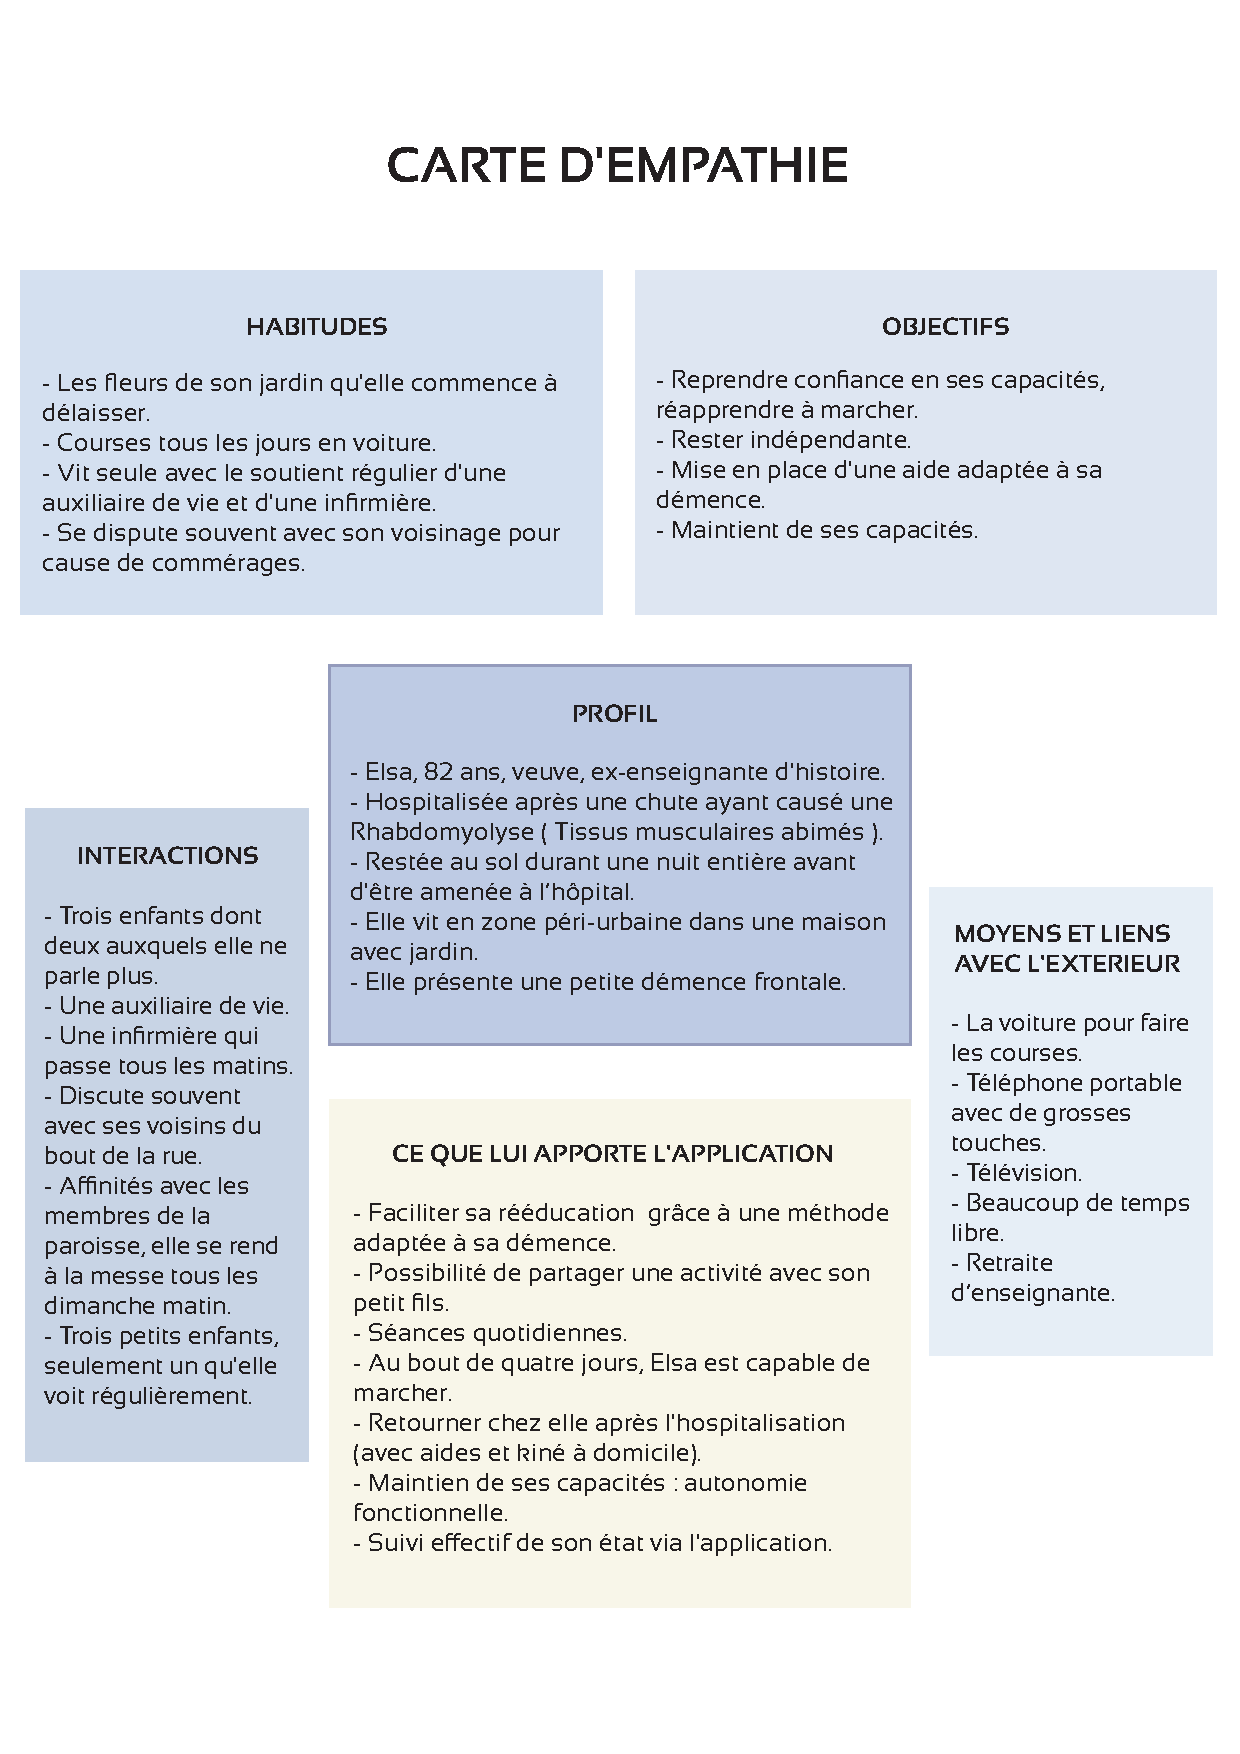
\includepdf{images/empathie_elsa}
\label{empathie_elsa}
	
	\subsubsection*{Imaginer et illustrer les cas d'utilisation}
La suite de la méthode de conception vient se servir des résultats des premières étapes. Il s'agit d'imaginer les différents cas d'utilisation de l'application. On va chercher à couvrir la totalité des fonctionnalités souhaitées de l'application dans différents contextes d'utilisation. Pour cela, on imagine des scénarios courts dans lesquels on pourra mettre en scène les utilisateurs imaginés lors de la séance de conception participative.

\paragraph{}Ces scénarios doivent comporter trois points~:
\begin{enumerate}
	\item un titre : permet de rapidement cerner la fonctionnalité ou le concept illustré.
	\item une description de la scène : elle permet de visualiser les acteurs présents, l'action en cours et les interactions.
	\item un commentaire : il s'agit d'expliquer ce qui se passe dans la scène, éventuellement comment on en est arrivé là, les objectifs en jeux ou l'intérêt de l'application ou du jeu.
\end{enumerate}

\paragraph{}Pour fournir des exemples de scénarios d'usage, je vais ici utiliser un travail issu d'un autre projet auquel j'ai participé. Il s'agissait ici de proposer une application pour aider à la rééducation de personnes lombalgiques. Le principal objectif est de faire bouger les patients : la douleur vient de l'inactivité et reprendre une activité physique est donc indispensable. Cette séance s'est déroulée notamment en présence d'un docteur en médecine spécialisé dans la lombalgie, Arnaud Dupeyron.

\begin{quotation}
	\emph{Slide Contexte} :\\
	\textbf{Description} : Paul est dans son canapé. Un proche lui recommande de se reposer.\\
	\textbf{Commentaire} : Il a mal au dos et est en arrêt maladie pour ça. Il aimerait ne plus avoir mal. Ses proches l’encouragent à se reposer, ne pas trop bouger.
	\paragraph{}
	\emph{Slide présentation par le médecin} :\\
	\textbf{Description} : Cabinet médical, Paul est entre les mains de son médecin. Il fait des exercices devant une kinect et un ordinateur.\\
	\textbf{Commentaire} : Le nouveau médecin qui va s’occuper du dos de Paul mesure les capacités de mouvement de Paul avec notre application. Il va conseiller à Paul de se remettre à bouger. Il lui déconseille d’être sédentaire et donc, il va lui recommander d’utiliser notre application chez lui afin de l’aider à se remettre en activité.
	\paragraph{}
	\emph{Slide suivi d’un patient} :\\
	\textbf{Description} : le médecin est devant son ordinateur, il consulte le profil de Paul et visualise ses capacités.\\
	\textbf{Commentaire} : l’application présente un bilan simplifié des capacités du patient. Notre application permet un suivi du patient par le médecin en remontant des informations sur l’endurance, la souplesse, la fréquence d’utilisation, des alertes … Mais le premier but de l’application c’est de faire bouger Paul.
\end{quotation}

	
	\subsubsection*{Création de storyboards}
Les storyboards sont des organisateurs graphiques sous la forme d'illustrations ou d'images affichées dans un ordre chronologique dans le but de pré-visualiser des séquences futures. Le storyboarding est utilisé dans le développement de logiciels pour mieux identifier leurs spécifications et les différentes étapes de l'expérience de l'utilisateur.
\paragraph{}
Dans notre cas, les storyboards sont construites à partir des scénarios d'usage conçu à l'étape précédente. Elles aident les utilisateurs à comprendre comment exactement l'application doit être utilisée au moyen d'une mise en scène de ces utilisations. C'est aussi un moyen de personnaliser l'expérience et de rapprocher les futurs utilisateurs de l'application, en la rendant plus accessible.
	
	\subsubsection*{Résumé et résultats}	 
Finalement, en quelques étapes bien définies, il est possible de passer d'une simple idée partagée à la production d'un document graphique mettant en scène toutes les possibilités d'utilisation de l'application idéale répondant aux principaux objectifs que l'on s'est fixés.

\paragraph{} Cette méthode met un fort accent sur une conception collaborative de la part des différents acteurs et met l'utilisateur et les impacts au centre du processus de conception. D'un point du vue du développement, on choisira une méthodologie AGILE mettant l'accent sur des échanges réguliers entre l'équipe de développement et les utilisateurs précédemment cités, afin de vérifier que le projet reste bien en corrélation avec leurs besoins. Elle permet entre autres de partager les connaissances et les compétences des participants, ce qui contribue à la qualité globale de la conception.

	\subsubsection{Différences et complémentarité des solutions}
Les deux approches empruntées pour aider à la conception de jeux sérieux pour la santé sont donc bien différentes. La première cherche plutôt à définir et enregistrer des savoirs qui seront utiles dans le processus de conception. La seconde, propose une méthodologie permettant de dynamiser les échanges entre les acteurs afin de répartir les savoirs.

\paragraph{} Il n'existe actuellement pas de méthode classique de conception spécifique à la création de serious games se distinguant par son efficacité. L'utilisation et la prise en compte de connaissances comme celles proposées en~\ref{boite_outils}, pourraient ainsi permettre de proposer des pistes intéressantes de conception. Si ce travail était poursuivi, en travaillant spécifiquement sur chaque type de jeu ou en enrichissant la base de contrôles possibles, il serait ainsi possible d'orienter efficacement la conception de l'application.

\paragraph{} Par ailleurs les deux approches proposées sont aussi compatibles. L'intégration de savoirs, s'ils font défaut à l'équipe de conception, peut permettre d'enrichir la pensée et les solutions envisagées. C'est aussi une manière d'envisager d'autres approches, comme utiliser le contrôle comme lien entre les composantes médicales et ludiques. La méthode de conception participative présentée peut trouver sa place dans le processus de conception avant l'utilisation de l'ensemble des outils. Ceux-ci pourront être plus justement utilisés lors de la phase de développement du l'application, en compléments des documents produits pendant la conception participative.
	

%		\subsubsection{}
%	
%	-travail avec les thérapeutes
%	-répondre aux objectifs thérapeutique par un gamedesign
%		- hammer \& Planks et l'équilibre (voir rapport d'anais)
%	-ajustement de la difficulté et lien avec la thérapie : impact des paramètres en terme de difficulté (équilibre et dos?)
